A EfficientNet-B0 iteratív tanításának eredményei négy lépésben először 1000 majd 5000 azután 10000 végül pedig 25000 képes halmazon. Ezelet a lépéseket 1k, 5k 10k 25k rövidítésekkel fogom jelölni.

%1K-----------------------------------------------------------------------------
\subsubsection{1k adathalmazon történő tanítás lépései EfficientNet-B0 modellen.}
  \begin{itemize} 
    \item Epoch 1/10 - train: 15/15 [00:02<00:00, 5.69it/s]
    \item Epoch 1: Train loss=4.9441, acc=0.0154 Val loss=4.7681, acc=0.0183
    \item Epoch 2/10 - train: 15/15 [00:01<00:00, 9.59it/s]
    \item Epoch 2: Train loss=4.0801, acc=0.1579 Val loss=4.5733, acc=0.0438
    \item Epoch 3/10 - train: 15/15 [00:01<00:00, 9.58it/s]
    \item Epoch 3: Train loss=3.4322, acc=0.3860 Val loss=4.3823, acc=0.0817
    \item Epoch 4/10 - train: 15/15 [00:01<00:00, 9.64it/s]
    \item Epoch 4: Train loss=2.8585, acc=0.6305 Val loss=4.1967, acc=0.1160
    \item Epoch 5/10 - train: 15/15 [00:01<00:00, 9.82it/s]
    \item Epoch 5: Train loss=2.2645, acc=0.8059 Val loss=4.0258, acc=0.1492
    \item Epoch 6/10 - train: 15/15 [00:01<00:00, 9.78it/s]
    \item Epoch 6: Train loss=1.8129, acc=0.9013 Val loss=3.8813, acc=0.1741
    \item Epoch 7/10 - train: 15/15 [00:01<00:00, 9.72it/s]
    \item Epoch 7: Train loss=1.4067, acc=0.9441 Val loss=3.7386, acc=0.1937
    \item Epoch 8/10 - train: 15/15 [00:01<00:00, 9.66it/s]
    \item Epoch 8: Train loss=1.0787, acc=0.9627 Val loss=3.6432, acc=0.2076
    \item Epoch 9/10 - train: 15/15 [00:01<00:00, 9.75it/s]
    \item Epoch 9: Train loss=0.8530, acc=0.9901 Val loss=3.5491, acc=0.2163
    \item Epoch 10/10 - train: 15/15 [00:01<00:00, 9.62it/s]
    \item Epoch 10: Train loss=0.6692, acc=0.9901 Val loss=3.4716, acc=0.2259
  \end{itemize}

\subsubsection{1k adathalmazon történő tanítás grafikonja EfficientNet-B0 modellen.}
  \begin{figure}[H]
    \centering
    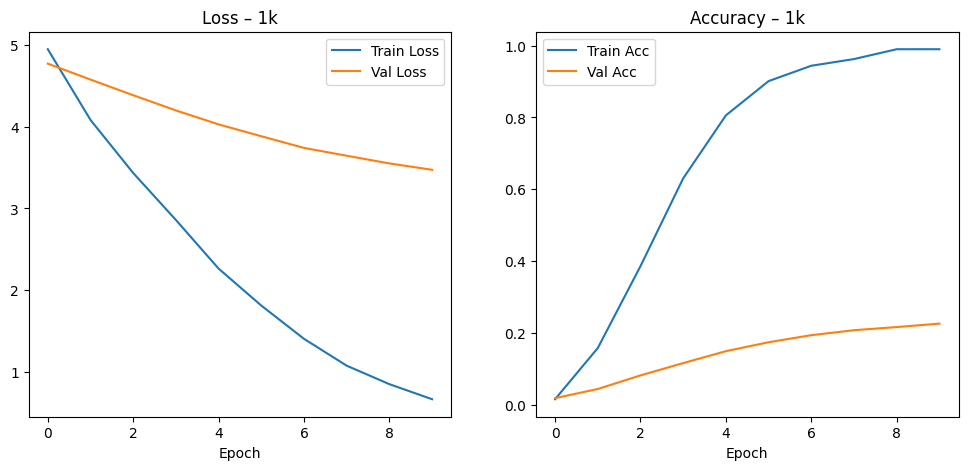
\includegraphics[width=1.0\textwidth]{images/phase03/phase03_EfficientNet-B0_1K_learning_curve.png}
    \caption{1k adathalmazon történő tanítás grafikonja EfficientNet-B0 modellen.}
    \label{fig:phase03_EfficientNet-B0_1K_learning_curve}
  \end{figure}

  \subsubsection{1k adathalmazon történő tanítás eredményei.}
    \begin{center}
      \begin{longtable}{l c}
      \caption{1k tanítás EfficientNet-B0-en.} \label{tab:phase03_EfficientNet-B0_1k} \\
      \toprule
      \textbf{Metrika} & \textbf{Érték} \\
      \midrule
      \endfirsthead
      \toprule
      \textbf{Metrika} & \textbf{Érték} \\
      \midrule
      \endhead
      Top-1 Accuracy & 0.2253 \\
      Top-5 Accuracy & 0.4770 \\
      Precision      & 0.2272 \\
      Recall         & 0.2487 \\
      F1-score       & 0.2176 \\
      Inference time & 24.75 sec \\
      \bottomrule
      \end{longtable}
    \end{center}


%5K-----------------------------------------------------------------------------
\subsubsection{5k adathalmazon történő tanítás lépései EfficientNet-B0 modellen.}
  \begin{itemize} 
    \item Epoch 1/10 - train: 77/77 [00:07<00:00, 10.56it/s]
    \item Epoch 1: Train loss=4.4209, acc=0.0767 Val loss=3.8978, acc=0.1752
    \item Epoch 2/10 - train: 77/77 [00:07<00:00, 10.93it/s]
    \item Epoch 2: Train loss=2.9662, acc=0.3721 Val loss=2.9698, acc=0.2947
    \item Epoch 3/10 - train: 77/77 [00:07<00:00, 10.92it/s]
    \item Epoch 3: Train loss=2.0437, acc=0.5734 Val loss=2.5196, acc=0.3684
    \item Epoch 4/10 - train: 77/77 [00:07<00:00, 10.82it/s]
    \item Epoch 4: Train loss=1.4631, acc=0.6991 Val loss=2.3690, acc=0.3936
    \item Epoch 5/10 - train: 77/77 [00:07<00:00, 10.97it/s]
    \item Epoch 5: Train loss=1.0588, acc=0.7974 Val loss=2.3003, acc=0.4036
    \item Epoch 6/10 - train: 77/77 [00:07<00:00, 10.99it/s]
    \item Epoch 6: Train loss=0.7509, acc=0.8817 Val loss=2.2574, acc=0.4137
    \item Epoch 7/10 - train: 77/77 [00:07<00:00, 10.84it/s]
    \item Epoch 7: Train loss=0.5345, acc=0.9337 Val loss=2.2344, acc=0.4189
    \item Epoch 8/10 - train: 77/77 [00:07<00:00, 10.91it/s]
    \item Epoch 8: Train loss=0.3647, acc=0.9643 Val loss=2.2295, acc=0.4211
    \item Epoch 9/10 - train: 77/77 [00:06<00:00, 11.05it/s]
    \item Epoch 9: Train loss=0.2604, acc=0.9812 Val loss=2.2593, acc=0.4182
    \item Epoch 10/10 - train: 77/77 [00:07<00:00, 10.95it/s]
    \item Epoch 10: Train loss=0.1879, acc=0.9890 Val loss=2.2372, acc=0.4233
  \end{itemize}

\subsubsection{5k adathalmazon történő tanítás grafikonja EfficientNet-B0 modellen.}
  \begin{figure}[H]
    \centering
    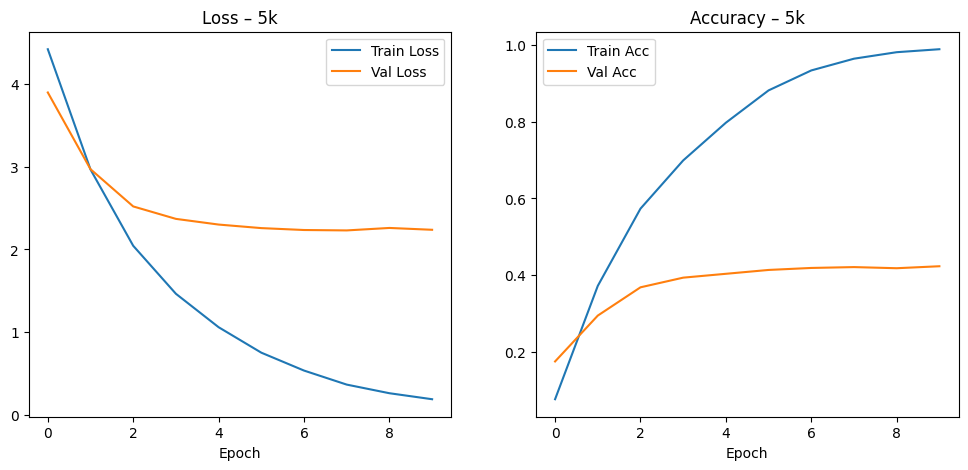
\includegraphics[width=1.0\textwidth]{images/phase03/phase03_EfficientNet-B0_5K_learning_curve.png}
    \caption{5k adathalmazon történő tanítás grafikonja EfficientNet-B0 modellen.}
    \label{fig:phase03_EfficientNet-B0_5K_learning_curve}
  \end{figure}

\subsubsection{5k adathalmazon történő tanítás eredményei.}
  \begin{center}
    \begin{longtable}{l c}
    \caption{5k tanítás EfficientNet-B0-en.} \label{tab:phase03_EfficientNet-B0_5k} \\
    \toprule
    \textbf{Metrika} & \textbf{Érték} \\
    \midrule
    \endfirsthead
    \toprule
    \textbf{Metrika} & \textbf{Érték} \\
    \midrule
    \endhead
    Top-1 Accuracy & 0.4209 \\
    Top-5 Accuracy & 0.7502 \\
    Precision      & 0.4014 \\
    Recall         & 0.4631 \\
    F1-score       & 0.4122 \\
    Inference time & 24.64 sec \\
    \bottomrule
    \end{longtable}
  \end{center}

%10K-----------------------------------------------------------------------------
\subsubsection{10k adathalmazon történő tanítás lépései EfficientNet-B0 modellen.}
  \begin{itemize} 
    \item Epoch 1/10 - train: 155/155 [00:14<00:00, 11.03it/s]
    \item Epoch 1: Train loss=3.9059, acc=0.1763 Val loss=2.8366, acc=0.3328
    \item Epoch 2/10 - train: 155/155 [00:14<00:00, 11.07it/s]
    \item Epoch 2: Train loss=2.2560, acc=0.4725 Val loss=2.2879, acc=0.4172
    \item Epoch 3/10 - train: 155/155 [00:13<00:00, 11.13it/s]
    \item Epoch 3: Train loss=1.5519, acc=0.6228 Val loss=2.0188, acc=0.4698
    \item Epoch 4/10 - train: 155/155 [00:13<00:00, 11.11it/s]
    \item Epoch 4: Train loss=1.1029, acc=0.7398 Val loss=1.9693, acc=0.4805
    \item Epoch 5/10 - train: 155/155 [00:13<00:00, 11.25it/s]
    \item Epoch 5: Train loss=0.7667, acc=0.8358 Val loss=2.0107, acc=0.4762
    \item Epoch 6/10 - train: 155/155 [00:13<00:00, 11.15it/s]
    \item Epoch 6: Train loss=0.5269, acc=0.9012 Val loss=1.9506, acc=0.4977
    \item Epoch 7/10 - train: 155/155 [00:13<00:00, 11.18it/s]
    \item Epoch 7: Train loss=0.3487, acc=0.9477 Val loss=1.9872, acc=0.4963
    \item Epoch 8/10 - train: 155/155 [00:13<00:00, 11.09it/s]
    \item Epoch 8: Train loss=0.2315, acc=0.9730 Val loss=2.0302, acc=0.4933
    \item Epoch 9/10 - train: 155/155 [00:13<00:00, 11.12it/s]
    \item Epoch 9: Train loss=0.1615, acc=0.9839 Val loss=2.0576, acc=0.4942
    \item Epoch 10/10 - train: 155/155 [00:14<00:00, 10.89it/s]
    \item Epoch 10: Train loss=0.1115, acc=0.9920 Val loss=2.0560, acc=0.5059
  \end{itemize}

\subsubsection{10k adathalmazon történő tanítás grafikonja EfficientNet-B0 modellen.}
  \begin{figure}[H]
    \centering
    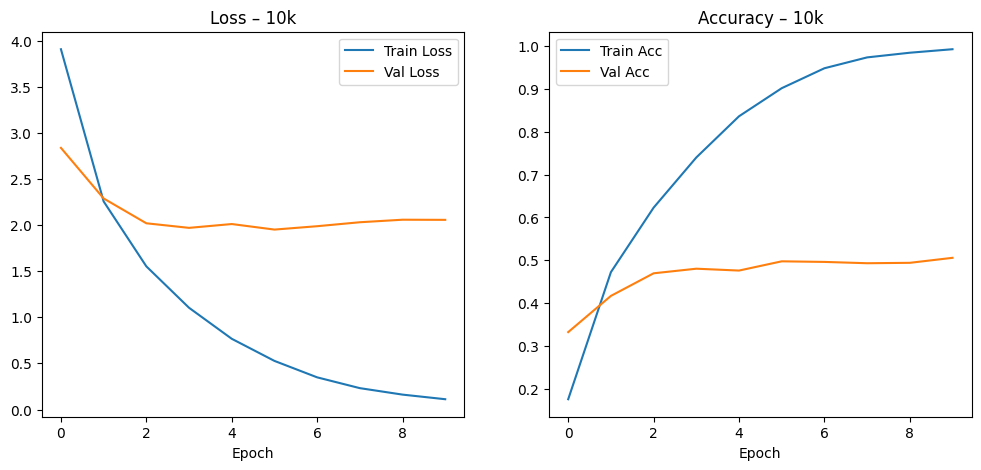
\includegraphics[width=1.0\textwidth]{images/phase03/phase03_EfficientNet-B0_10K_learning_curve.png}
    \caption{10k adathalmazon történő tanítás grafikonja EfficientNet-B0 modellen.}
    \label{fig:phase03_EfficientNet-B0_10K_learning_curve}
  \end{figure}

\subsubsection{10k adathalmazon történő tanítás eredményei.}
  \begin{center}
    \begin{longtable}{l c}
    \caption{10k tanítás EfficientNet-B0-en.} \label{tab:phase03_EfficientNet-B0_10k} \\
    \toprule
    \textbf{Metrika} & \textbf{Érték} \\
    \midrule
    \endfirsthead
    \toprule
    \textbf{Metrika} & \textbf{Érték} \\
    \midrule
    \endhead
    Top-1 Accuracy & 0.4982 \\
    Top-5 Accuracy & 0.8060 \\
    Precision      & 0.4552 \\
    Recall         & 0.5263 \\
    F1-score       & 0.4728 \\
    Inference time & 24.67 sec \\
    \bottomrule
    \end{longtable}
  \end{center}

%25K-----------------------------------------------------------------------------
\subsubsection{25k adathalmazon történő tanítás lépései EfficientNet-B0 modellen.}
  \begin{itemize} 
    \item Epoch 1/10 - train: 391/391 [00:34<00:00, 11.47it/s]
    \item Epoch 1: Train loss=2.9738, acc=0.3201 Val loss=2.0269, acc=0.4593
    \item Epoch 2/10 - train: 391/391 [00:34<00:00, 11.33it/s]
    \item Epoch 2: Train loss=1.6467, acc=0.5703 Val loss=1.7581, acc=0.5119
    \item Epoch 3/10 - train: 391/391 [00:34<00:00, 11.42it/s]
    \item Epoch 3: Train loss=1.1533, acc=0.6915 Val loss=1.7306, acc=0.5289
    \item Epoch 4/10 - train: 391/391 [00:34<00:00, 11.47it/s]
    \item Epoch 4: Train loss=0.8124, acc=0.7856 Val loss=1.6478, acc=0.5532
    \item Epoch 5/10 - train: 391/391 [00:34<00:00, 11.40it/s]
    \item Epoch 5: Train loss=0.5515, acc=0.8632 Val loss=1.7309, acc=0.5466
    \item Epoch 6/10 - train: 391/391 [00:33<00:00, 11.57it/s]
    \item Epoch 6: Train loss=0.3730, acc=0.9144 Val loss=1.7486, acc=0.5584
    \item Epoch 7/10 - train: 391/391 [00:34<00:00, 11.47it/s]
    \item Epoch 7: Train loss=0.2451, acc=0.9501 Val loss=1.8576, acc=0.5498
    \item Epoch 8/10 - train: 391/391 [00:34<00:00, 11.42it/s]
    \item Epoch 8: Train loss=0.1662, acc=0.9693 Val loss=1.9198, acc=0.5533
    \item Epoch 9/10 - train: 391/391 [00:33<00:00, 11.52it/s]
    \item Epoch 9: Train loss=0.1234, acc=0.9787 Val loss=2.0300, acc=0.5401
    \item Epoch 10/10 - train: 391/391 [00:34<00:00, 11.36it/s]
    \item Epoch 10: Train loss=0.0963, acc=0.9841 Val loss=1.9793, acc=0.5616
  \end{itemize}

\subsubsection{25k adathalmazon történő tanítás grafikonja EfficientNet-B0 modellen.}
  \begin{figure}[H]
    \centering
    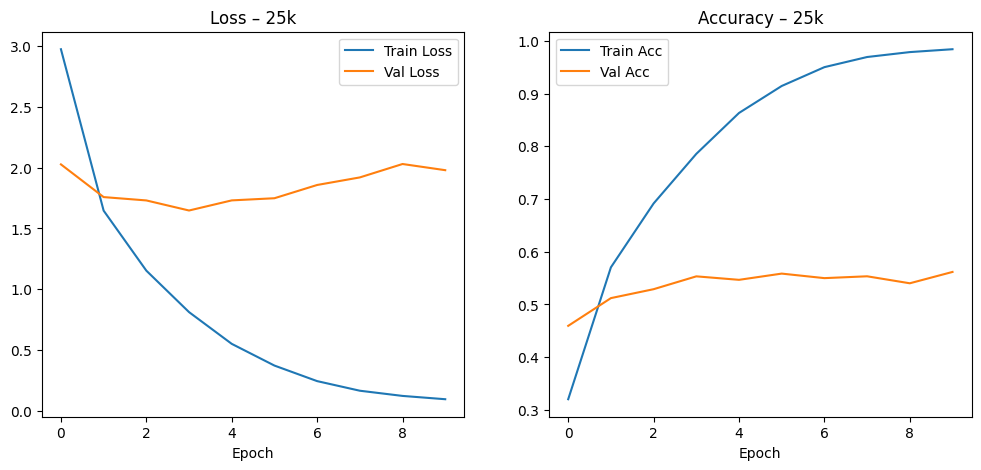
\includegraphics[width=1.0\textwidth]{images/phase03/phase03_EfficientNet-B0_25K_learning_curve.png}
    \caption{25k adathalmazon történő tanítás grafikonja EfficientNet-B0 modellen.}
    \label{fig:phase03_EfficientNet-B0_25K_learning_curve}
  \end{figure}

\subsubsection{25k adathalmazon történő tanítás eredményei.}
\begin{center}
  \begin{longtable}{l c}
  \caption{25k tanítás EfficientNet-B0-en.} \label{tab:phase03_EfficientNet-B0_25k} \\
  \toprule
  \textbf{Metrika} & \textbf{Érték} \\
  \midrule
  \endfirsthead
  \toprule
  \textbf{Metrika} & \textbf{Érték} \\
  \midrule
  \endhead
  Top-1 Accuracy & 0.5630 \\
  Top-5 Accuracy & 0.8460 \\
  Precision      & 0.5210 \\
  Recall         & 0.6069 \\
  F1-score       & 0.5460 \\
  Inference time & 24.78 sec \\
  \bottomrule
  \end{longtable}
\end{center}

\subsubsection{EfficientNet-B0 iteratív tanítás összefoglaló}
  \begin{center}
    \begin{longtable}{lllllll}
    \caption{Összehasonlító táblázat a EfficientNet-B0 iteratív tanításáról.}\label{tab:phase3_EfficientNet-B0_summary_table}\\
    \toprule
    Minta & Top-1 & Top-5 & Precision & Recall & F1 & Time(s) \\
    \midrule
    \endfirsthead
    \toprule
    Minta & Top-1 & Top-5 & Precision & Recall & F1 & Time(s) \\
    \midrule
    \endhead
    1k & 0.2253 & 0.4770 & 0.2272 & 0.2487 & 0.2176 & 24.75 \\
    5k & 0.4209 & 0.7502 & 0.4014 & 0.4631 & 0.4122 & 24.64 \\
    10k & 0.4982 & 0.8060 & 0.4552 & 0.5263 & 0.4728 & 24.67 \\
    25k & 0.5630 & 0.8460 & 0.5210 & 0.6069 & 0.5460 & 24.78 \\
    \bottomrule
    \end{longtable}
  \end{center}
  
  \subsubsection{Összehasonlító grafikon a EfficientNet-B0 iteratív tanításáról.}
  \begin{figure}[H]
    \centering
    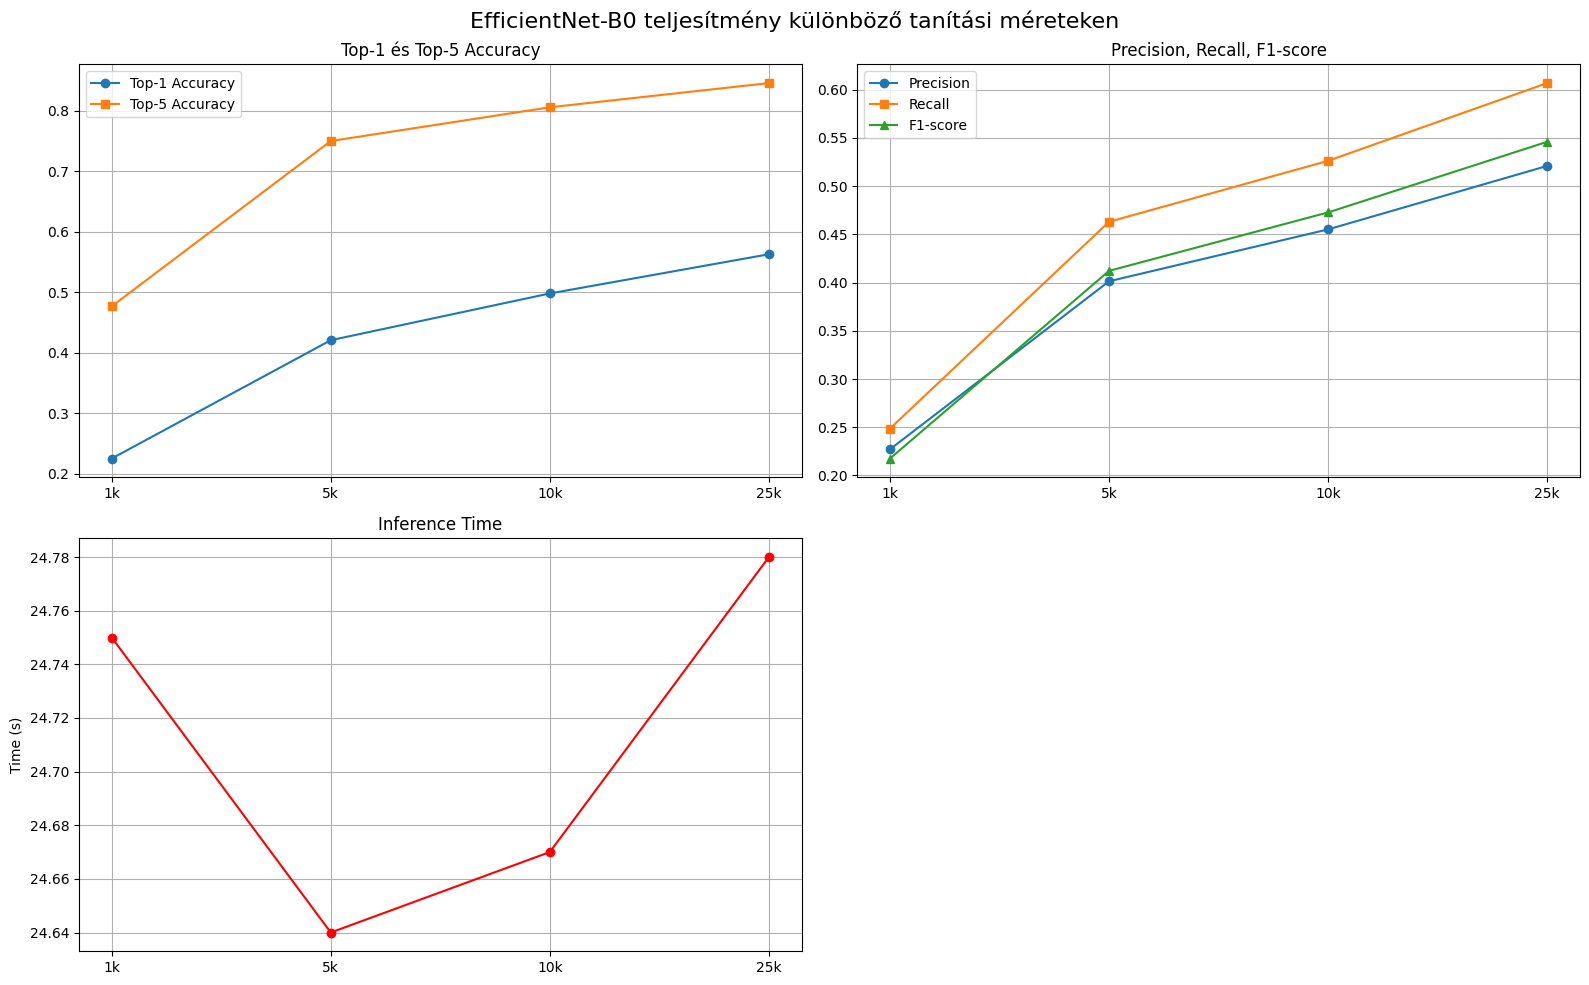
\includegraphics[width=1.0\textwidth]{images/phase03/phase03_EfficientNet-B0_summary_curve.png}
    \caption{Összehasonlító grafikon a EfficientNet-B0 iteratív tanításáról.}
    \label{fig:phase03_EfficientNet-B0_summary_curve}
  \end{figure}

  \subsubsection{Összehasonlító metrika grafikon a EfficientNet-B0 iteratív tanításáról.}
  \begin{figure}[H]
    \centering
    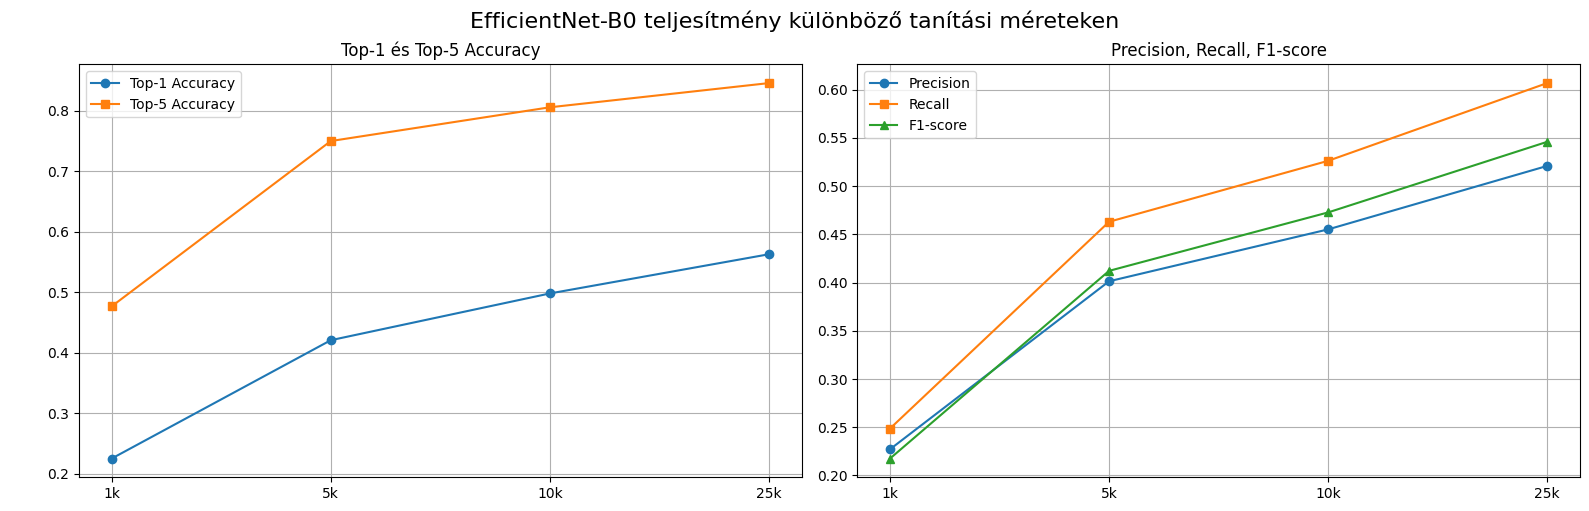
\includegraphics[width=1.0\textwidth]{images/phase03/phase03_EfficientNet-B0_summary_curve_metrics.png}
    \caption{Összehasonlító metrika grafikon a EfficientNet-B0 iteratív tanításáról.}
    \label{fig:phase03_EfficientNet-B0_summary_curve_metrics}
  \end{figure}

  \subsubsection{Összehasonlító idő grafikon a EfficientNet-B0 iteratív tanításáról.}
  \begin{figure}[H]
    \centering
    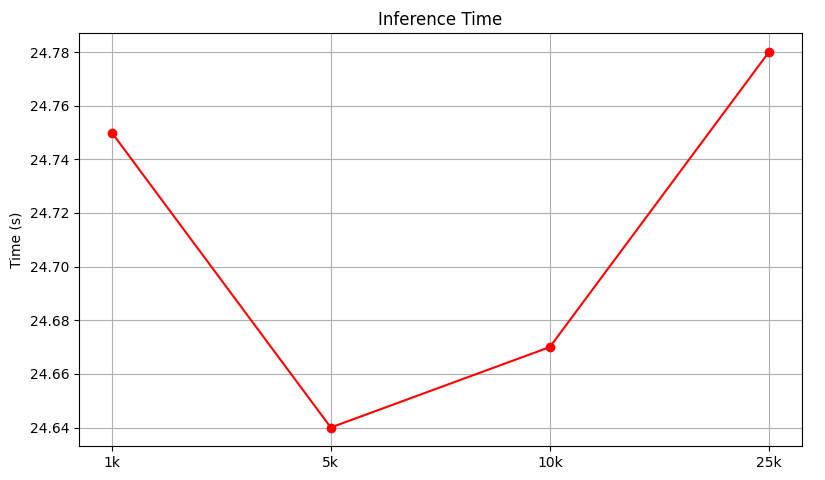
\includegraphics[width=1.0\textwidth]{images/phase03/phase03_EfficientNet-B0_summary_curve_time.png}
    \caption{Összehasonlító idő grafikon a EfficientNet-B0 iteratív tanításáról.}
    \label{fig:phase03_EfficientNet-B0_summary_curve_time}
  \end{figure}

  \subsubsection{Összehasonlító grafikon a EfficientNet-B0 iteratív tanításáról 10 EPOCH-on keresztül.}
  \begin{figure}[H]
    \centering
    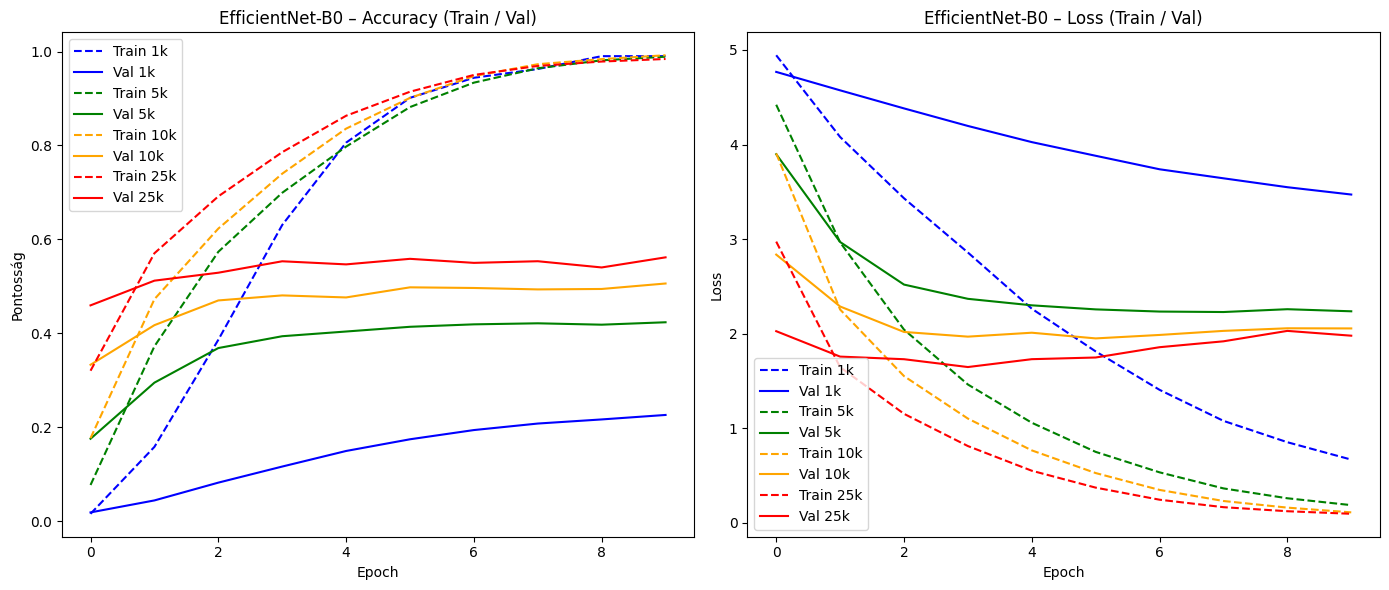
\includegraphics[width=1.0\textwidth]{images/phase03/phase03_EfficientNet-B0_learning_summary_curve.png}
    \caption{Összehasonlító grafikon a EfficientNet-B0 iteratív tanításáról 10 EPOCH-on keresztül.}
    \label{fig:phase03_EfficientNet-B0_learning_summary_curve}
  \end{figure}

  \subsubsection{Összehasonlító Confusion Matrix a EfficientNet-B0 iteratív tanításáról.}
  \begin{figure}[H]
    \centering
    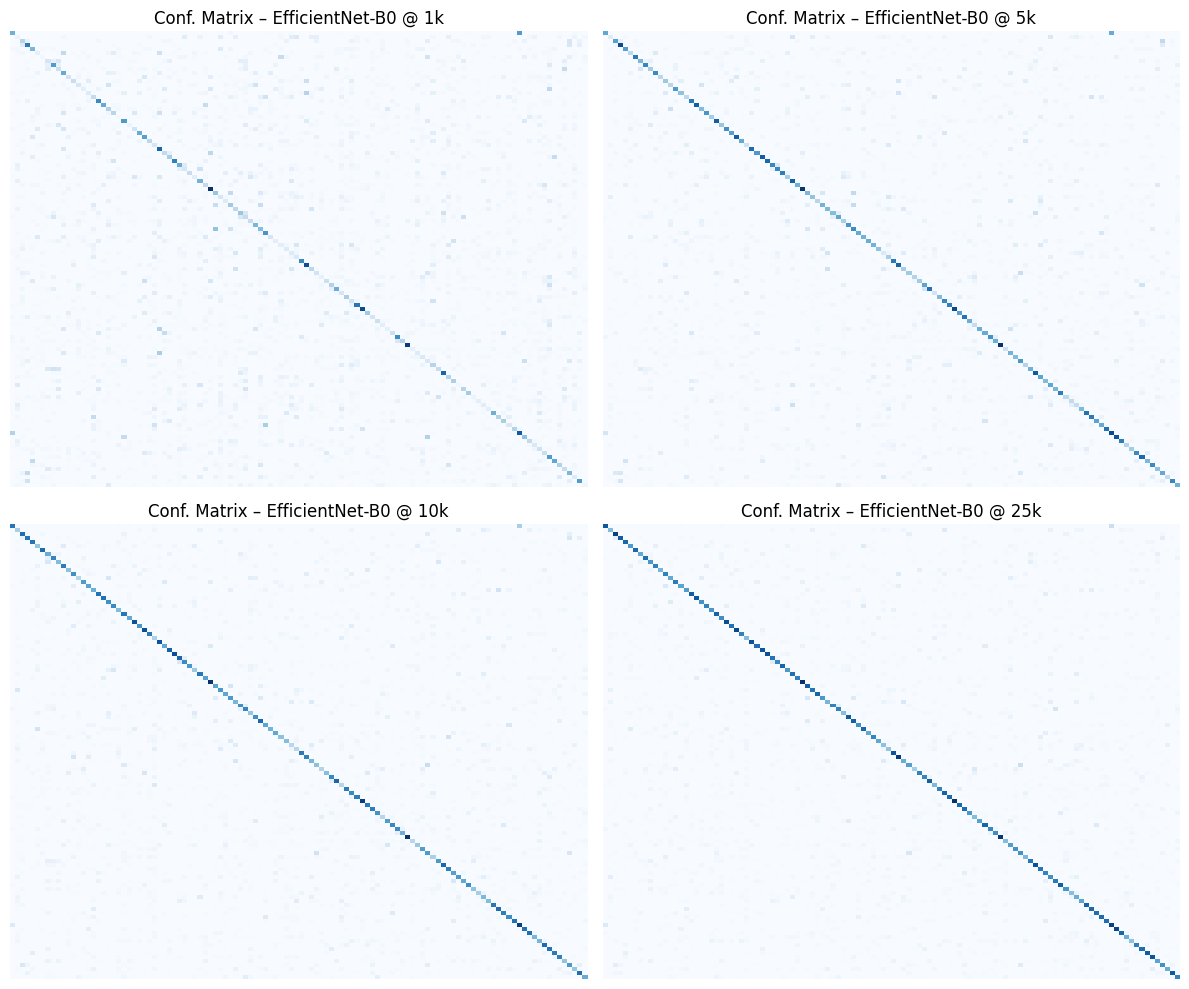
\includegraphics[width=1.0\textwidth]{images/phase03/phase03_EfficientNet-B0_Confusion_Matrix_summary_curve.png}
    \caption{Összehasonlító Confusion Matrix a EfficientNet-B0 iteratív tanításáról 10 EPOCH-on keresztül.}
    \label{fig:phase03_EfficientNet-B0_Confusion_Matrix_summary_curve}
  \end{figure}